\begin{frame}[fragile]{Using UHD from C++ (2/5)}

\textbf{\textcolor{red}{NEEL FIXME (clean up path names and explanation)}}

\footnotesize

\begin{itemize}
    \item \textbf{\textcolor{DarkBlue}{Step 2: Use the example CMakeLists.txt}}
\end{itemize}

\begin{quote}
\footnotesize
There is an example \texttt{CMakeLists.txt} with UHD examples.
It already contains the required configuration to locate UHD libraries,
include directories and link your C++ application against the UHD API.

Copy this file into the directory containing your C++ source file.
\end{quote}

\scriptsize

\begin{Verbatim}[xleftmargin=3em,breaklines,breaksymbolleft={},breaksymbolright={}]
cp /home/ettus-kb-xubuntu24-04-3/workarea/uhd/host/examples/init_usrp/CMakeLists.txt .
\end{Verbatim}

\vspace{0.2cm}

\begin{center}
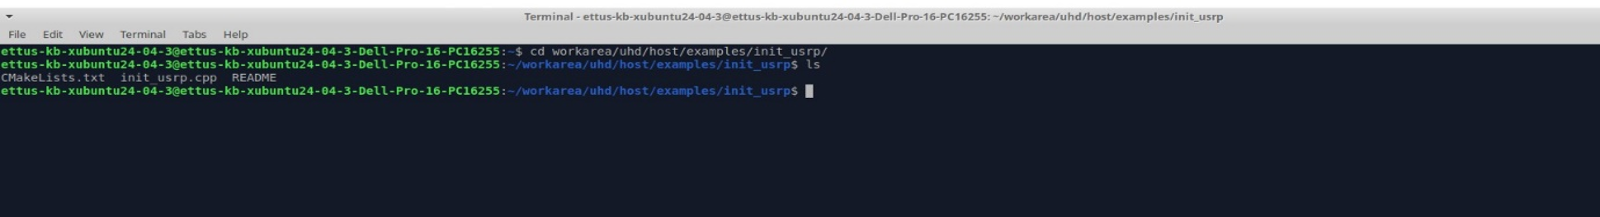
\includegraphics[width=0.75\linewidth]{latex/jpg_png/image_c++_3.png}

\vspace{0.2cm}

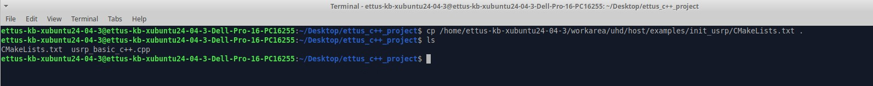
\includegraphics[width=0.85\linewidth]{latex/jpg_png/image_c++_4.png}
\end{center}

\end{frame}